\section{Crawling}

\subsection{Principi di base}

\paragraph{Insiemi di nodi in una visita}
All'interno di un processo di crawling, si distinguono 
tre insiemi di nodi 
\begin{itemize}
    \item $U$: nodi sconosciuti 
    \item $F$: frontiera, ovvero nodi che sono conosciuti ma non ancora visitati
    \item $V$: nodi visitati
\end{itemize}
Una visita del web opera scegliendo un nodo della frontiera, 
aggiungendolo ai visitati, e aggiungendo i siti raggiungibili da esso alla frontiera.

In una visita di un grafo classica, gli insiemi $U$ e $F$ coincidono nel secondo.
\begin{remark}
    Teoricamente una visita potrebbe esaurire la frontiera, 
    praticamente non finisce mai, a parte in rari casi.
\end{remark}

\paragraph{Inizializzazione frontiera}
La frontiera va inizializzata, tipicamente si scelgono siti web popolari, 
per esempio giornali etc. In generale si considerano \emph{semi} di inizializzazione, 
ovvero un insieme di siti web scelti da umani, che sono promettenti.

La scelta del seme governa l'esplorazione della frontiera, 
verranno scelti infatti prima siti più vicini ai siti di inizializzazione.

Un'altra strada per la frontiera è scegliere a priori un insieme di siti 
web, e considerarla direttamente come frontiera, tralasciando i siti 
raggiungibili da essi. 

\subsection{Strutture dati}

\paragraph{Strutture in memoria}
Sono cruciali le strutture usate per memorizzare i nodi visitati 
e la frontiera.

Mantenere i visitati in una hashtable è ragionevole, non lo è 
per la frontiera, tipicamente di ordini di grandezza più grande dell'insieme $V$.

Limitare la grandezza della frontiera è cruciale, si potrebbere preferire 
i link iniziali in una pagina piuttosto che quelli a fondo. Oppure limitare 
il numero massimo di pagine estratte da un singolo dominio o considerare 
un limite alla profondità all'interno di un singolo sito web.

\paragraph{Scelta del prossimo nodo}
Ciò che determina il comportamento una visita di crawling è 
la scelta del prossimo nodo della frontiera. Una scelta ragionevole 
potrebbe essere una visita in ampiezza a partire dalla frontiera iniziale.
L'assunzione è che pagine di qualità puntino ad altre pagine di qualità.

Operare in profondità non funziona, significherebbe continuare a scendere 
all'infinito, al contrario di una classica DFS che termina e si \emph{torna indietro} 
con la ricorsione. Questo perchè i siti non visitati sono praticamente infiniti.

Criteri più sofisticati possono associare una sorta di priorità alle pagine. 
Tali criteri sono legati ai contenuti delle pagine, alla struttura dell'url, 
alcuni esempi sono:
\begin{itemize}
    \item Url corti, con l'assunzione che i livelli siano separati da un backslash;
    \item Url fuori dal sito corrente;
    \item Parole chiave di interesse all'interno dell'url;
    \item Utilizzo il contenuto della pagina corrente per avere informazioni 
    sulla pagina successiva.
\end{itemize}
In questo caso si utilizza una coda a priorità, con qualche valore di priorità 
associato ad ogni nodo.

\begin{remark}
    In questo paragrafo si sta assumendo un contesto single thread, ovviamente nella realtà si 
    utilizzerà un approccio multithread, e molti fattori, quali latenza, 
    tempi di risposta, race condition, influenzano sull'ordine di visita effettivo.
\end{remark}

\subsubsection{Esempio strutture dati}

\paragraph{Visti hashati}
Una prima idea per mantenere l'insieme $V$ è non memorizzare url completi ma una certa firma digitale 
di essi. 

Consideriamo ad esempio una funzione di hash:
$$f : \mathit{URL} \longrightarrow 2^{64} = \{0, \dots, 2^{64-1}\}$$
È possibile che due url collidano, creando errori sui positivi, ovvero un 
url non davvero visitato viene visto come già esplorato.

Solitamente le collisioni non importano, ma, dati $k$ elementi contenuti 
nella struttura, data una funzione di hash buona, tipicamente il numero di collisioni 
è dell'ordine di $\frac{k^2}{2n}$, dove $n$ è la grandezza del codominio. 

Nella pratica quindi, funzioni di hash come $f$, non creano un numero 
spiacevole di collisioni.
\begin{remark}
    Una tabella di firme è molto più efficiente di mantenere i dati effettivi, 
    basti pensare a problemi di allocazione di memoria inefficiente, frammentazione 
    etc.
    Pagare il prezzo dei conflitti, implica risparmiare molti problemi e spazio.\\
    Mantenere una tabella di firme significa di fatto mantenere in memoria strutture 
    più piccole dell'information theoretical lower bound, pagando il prezzo delle collisioni.
\end{remark}

\paragraph{Database NoSQL}
Sono  database che memorizzano entry chiave valore, 
un esempio è \emph{RocksDB}. Se ordinati sono implementazioni efficienti di B-Tree, 
altrimenti di dizionari classici, in parte memorizzati su disco. 

Si utilizzano anche LSM-Tree, alberi che dividono per livelli le chiavi e mantengono 
chiavi utilizzate di frequente all'inizio, spostando chiavi poco frequenti nei 
livelli più bassi.

\subsection{Crivelli}

Un crivello è una struttura dati che accetta le seguenti primitive: 
\begin{itemize}
    \item \emph{add(u)}: aggiunge un url alla struttura;
    \item \emph{get()}: preleva un elemento dalla struttura. 
\end{itemize}
Un crivello ha un aspetto insiemistico, ovvero ricorda cosa è stato inserito 
o no, gestisce anche l'ordine in cui restituisce i dati, tipicamente 
si considera una visita in ampiezza. 

Un' implementazione base è un' hashtable in memoria, per i già visti, ovvero $V \cup F$, 
e una coda in memoria per gestire l'ordine di visita, BFS nel caso di una coda classica.

\begin{remark}
    È necessario comunque del processing degli url estratti dal crivello, ad esempio, 
    potremmo ordinarli per dominio, in modo da raggruppare richieste allo stesso sito.
\end{remark}

\paragraph{Implementazione}
È già stata accennata la possibilità di avere una hashtable più una coda. 
L'hashtable potrebbe, come introdotto a sottosezione precedente, solo le firme degli url, in modo da ridurre lo spazio in memoria necessario.

\paragraph{Graceful degradation}
È importante garantire il \emph{graceful degradation}, ovvero, il sovraccarico della 
struttura ne peggiora le performance ma non fa crollare l'intero processo. 
Una struttura dati classica, come una hashtable, non garantisce questa proprietà, 
al termine della memoria essa fallisce.

\subsubsection{Filtri di Bloom}
Un filtro di Bloom è un dizionario approssimato, che garantisce una certa probabilità di errore positivo assumendo un certo upper bound al numero di chiavi inserite. 

L'impronta in memoria di un filtro di questo tipo è costante, non varia quindi al variare 
del carico della struttura.

\paragraph{Funzionamento}

Sia $b$ un vettore di $m$ bit, sia $d$ il parametro che regola la precisione del filtro,
e $f_i : U \rightarrow m, 0 < i < d$ funzioni di hash che mappano un elemento dell'universo 
in un indice del vettore. 

Le primitive disponibili sono, dato $x \in U$: 
\begin{itemize}
    \item \emph{add(x)}: imposto ad uno le posizioni date dalle funzioni di hash, 
    ovvero $f_0(x), \dots, f_{d-1}(x)$;
    \item \emph{contains(x)}: restituisco l'and logico delle posizioni $b[f_i(x)]$.
\end{itemize}

L'operazione contains restituisce zero se e solo se $x$ non è stato inserito nel filtro. 
Un risultato positivo però può significare che $x$ sia stato inserito oppure che 
inserimenti precedenti abbiano settato ad uno tutte le celle relative agli hash di $x$.

\paragraph{Probabilità di falsi positivi}
Se fissiamo $d$ ad uno non si sta guadagnando rispetto ad una classica tabella di hash.
Più $d$ è grande, più sono improbabili i falsi positivi, ma più uni si vanno ad aggiungere, quindi i falsi positivi aumentano.

Bisogna quindi trovare un tradeoff tra $m$ e $d$ per minimizzare la probabilità di falsi positivi.
Si considera ora un $n$, ovvero il numero di chiavi inserite. 

Si ottiene che la probabilità di un falso positivo equivale a $\frac{1}{2}^d$ e la 
dimensione $m = 1.44 dn$. 
Questo implica che fissata una precisione e il numero di chiavi massimo, si può ottenere lo 
spazio necessario, similmente, fissato $m$ e $n$ si può ottenere la precisione ottenuta.

\begin{remark}
    La struttura ha degrado grazioso, infatti, eccedendo $n$ l'analisi di precisione non vale più e 
    i falsi positivi aumentano. Si nota anche che sotto la soglia $n$ la probabilità di falsi 
    positivi diminuisce. 
    La struttura non fallisce, peggiora in precisione fino a che è satura, restituendo sempre positivo.
\end{remark}
\begin{remark}
    Gli accessi in cache sono pessimi per quanto riguarda un filtro di bloom, 
    dovendo controllare celle di memoria non correlate e sostanzialmente casuali, 
    quindi con poca probabilità di essere in cache.
\end{remark}
\begin{remark}
    I risultati negativi in media accedono a solo due celle.
\end{remark}

\paragraph{Blocked Bloom filter}
Si può pensare di dividere un filtro di Bloom in due filtri più piccoli di dimensione $1.44d\frac{n}{2}$ ciascuno.
Una funzione $g$ sceglie quale filtro scegliere, poi, si inserisce l'elemento nel filtro selezionato.

La divisione permette di mantenere i filtri in cache e velocizzare il tutto. 
Un'analisi avanzata individua un degrado di precisione. Questo perché alcuni filtri 
mantengono poche chiavi, ed altri saranno più sovraccarichi.

\paragraph{Calcolo funzioni di hash}
Supponendo di avere due funzioni di hash $h(x)$ e $g(x)$, siano $a = h(x)$ e 
$b = g(x)$, considerando l'i-esima funzione di hash come $ai + b$, 
l'analisi sulla precisione di falsi positivi rimane valida. 
\begin{remark}
    Il calcolo fatto in questo modo è estremamente più efficiente di calcolare 
    $d$ funzioni separate. 
\end{remark}

\subsubsection{LMS tree}
Un \emph{Log-Structure-Merge} tree memorizza file di log in cui si scrive solo in append. 

A differenza di un classico \emph{B-tree}, i registri non cambiano.
Questi alberi funzionano molto bene quando si scrive molto e legge poco.

\paragraph{Livelli}
L'idea di base di un \emph{LMS} tree è avere un certo numero di livelli nella struttura 
dati. Idealmente i vari livelli possono essere mantenuti in mezzi di memorizzazione 
differenti. 
Si assume ora che il primo livello sia in memoria, in una struttura classica 
come un B-tree e i successivi su disco come registri di coppie chiave-valore ordinate. 

Ogni livello ha memorizzate un certo numero di coppie chiave-valore, ed ogni livello successivo occupa 
dieci volte più del precedente. 

\paragraph{Ricerca}
Per trovare una chiave, si cerca nei livelli in maniera sequenziale, 
una volta individuata, al livello più alto possibile\footnote{Potrebbe comparire 
anche in livelli successivi, visto che si ammettono duplicati}, si restituisce.
Visto che le chiavi sono ordinate, si potrebbe effettuare una ricerca 
dicotomica\footnote{Bisogna stare attenti al tipo di memoria, a volte accessi sequenziali 
sono molto più veloci di accessi aleatori, un esempio è nel nastro.}.

\paragraph{Inserimento}
L'aggiunta all'albero inserisce la chiave al livello zero. Se la chiave non è presente il B-tree sale di dimensione, se eccede la dimensione massima: 
si considera un segmento contiguo di chiavi e si fondono con il livello uno\footnote{La fusione 
è molto veloce essendo le due strutture ordinate}.
Si procede fino a che non si trova un livello che riesce a mantenere le chiavi. 
Se si raggiunge l'ultimo livello, se ne crea uno nuovo. 

Il principio di base è che le fusioni dei livelli, che sono molto costose, avvengono sempre 
più raramente allo scendere nell'albero.

\paragraph{Rimozione}
La rimozione consiste nella ricerca della chiave e nella sostituzione del suo 
valore con una \emph{tombstone}. Una ricerca successiva troverà questo valore e capirà 
che la chiave è stata rimossa.

\paragraph{Frammentazione livelli}
Ogni livello nella pratica è frammentato in tanti file piccoli. Questo offre 
molti vantaggi, ad esempio operazioni di merge parallele. Inoltre, favorisce 
l'evitare collisioni di concorrenza. 

La ricerca poi è più veloce, poiché è 
possibile mantenere un indice sparso, con un sottoinsieme di chiavi, con puntatori 
ai frammenti relativi alla chiave. Ogni livello ha poi un filtro di Bloom.
La ricerca quindi testa il filtro e se la risposta è negativa si procede al 
livello successivo, altrimenti, si controlla l'indice sparso in ricerca dicotomica, 
e si procede sequenzialmente dalla maggior chiave minore uguale di quella ricercata.

\subsubsection{Crivello offline} 
Si mantengono solo file su disco e non strutture in memoria. 
I file vengono ordinati e fusi spesso. In particolare, si hanno a disposizione: 
\begin{itemize}
    \item \emph{Z}: url già visti, $V \cup F$
    \item \emph{F}: frontiera, ovvero gli url da visitare
    \item \emph{A}: file che accumula gli url incontrati durante la visita
\end{itemize}

All'inizio $Z$ ed $F$ sono inizializzati con il seme ed $A$ è vuoto.
Durante la visita si estrae con qualche criterio da $F$, accumulando in $A$, 
quando si esaurisce il primo o il secondo è pieno:
\begin{enumerate}
    \item $A$ viene ordinato e deduplicato, diventa $A^\prime$;
    \item $Z$ diventa $Z^\prime$ pari all'unione di  $A^\prime$ e $Z$: 
    durante la fusione gli url che compaiono in $A^\prime$ ma non in $Z$ vengono 
    aggiunti ad $F$.
\end{enumerate}

Il punto due ha complessità lineare, visto che i due file sono ordinati, 
l'ordinamento di $A^\prime$ disordina gli url per quanto riguarda l'ordine di accodamento, 
per ovviare al problema si potrebbe mantenere nel file oltre che l'url, la posizione originale
di accodamento, in modo da riordinarli una volta accodati ad $F$.

$Z$ potrebbe contenere firme al posto di url, in questo caso $A$, che contiene url, 
va ordinato indirettamente per firma.

Al crescere della frontiera il crivello diventa lento ma non si blocca, ha perciò graceful 
degradation.

\paragraph{LRU cache}
Può essere una buona idea anteporre al crivello una cache LRU, questo rimuove 
molti duplicati, infatti se un url è all'interno della cache è già stato inserito 
all'interno del crivello. \\
Ogni tanto un url verrà inserito più volte, perché finito fuori dalla cache.

\subsection{Quasi duplicati}
Per molteplici ragioni, è possibile incontrare spesso le stesse pagine, 
per esempio, la stessa pagina con http e https, pagine che differiscono per una 
sola data, etc.\\
È necessario un sistema che decida se due pagine sono quasi identiche.

\paragraph{Digest}
Si puo generare un digest dalla pagina web, buttando via alcuni elementi, 
per esempio i tag html, le maiuscole, etc.
Si può anche campionare la pagina in qualche intervallo e memorizzare solo 
i campionamenti.
Una volta generati questi digest saranno inseriti in un filtro di Bloom.

\paragraph{SimHash}
L'idea di base è generare hash simili per testi simili. La distanza tra due testi 
si misura in distanza di Hamming.
Si risolvono problemi come ad esempio il considerare due pagine diverse per un 
singolo errore ortografico.

A partire dal testo si ottengono delle feature da esso. Un esempio potrebbe essere 
estrarre le parole, oppure considerare tre-gram da esso, ovvero sotto-sequenze di tre 
caratteri o magari tre parole alla volta, etc.
N-gram corti implicano il non considerare troppo importanti errori di ortografia.

Siano ora $s \in S$ le feature estratte e $h : \mathit{Stringhe} \rightarrow 2^b$ funzione 
di hash.
Consideriamo ora il valore di hash per ogni feature, $h(s)$, l'hash finale del documento 
si ottiene contando la maggioranza per ogni bit degli hash delle feature, per esempio: 
\begin{itemize}
    \item $s_0$ : $1,0,1,1,0$;
    \item $s_1$ : $0,1,0,0,1$;
    \item $s_2$ : $0,1,0,1,1$;
\end{itemize}
L'hash finale del documento sarà: $0, 1, 0, 1, 1$

Il calcolo effettuato in questo modo sistema i casi di poche differenze tra i testi, 
dipende ovviamente dalle feature che si considerano, ma è auspicabile che poche 
feature differenti tra due documenti non modifichino i voti di maggioranza, oppure, che influiscano su pochi bit. 

\subsection{Politeness}

Dal punto di vista etico, una persona che mette una pagina sul web 
deve accettare che sarà visitata, da umani. 
La visita e l'indicizzazione automatica tramite crawler non dovrebbe 
continuare per periodi troppo prolungati.

\paragraph{Politeness assoluta}
Intervallare di un certo numero di secondi le richieste consecutive ad 
un sito, oppure allo stesso ip. Esempio, faccio 10 richieste, pausa di qualche secondo, altre 10 richieste.

\paragraph{Politeness relativa}
Per un certo intervallo di tempo scarico tutto quello che posso. Poi mi 
adatto in base a come la pagina ha risposto, ad esempio, 
scarico per un secondo tutto quello che riesco, ma la pagina impiega 
10 secondi a rispondere, aspetto quindi 30 secondi prima di effettuare 
una nuova richiesta.

Potrei usare HTTP 1.1, per mantenere aperta la connessione. 

\begin{remark}
    È necessaria un'architettura multiflusso per raccogliere dati 
    da molti siti contemporaneamente, altrimenti si aspetterebbe molto 
    per ragioni di politeness e si diventerebbe troppo dipendenti 
    dall'ordine della coda dei siti da visitare, infatti, dovrei aspettare 
    se il prossimo sito fosse nello stesso dominio di quello attuale, no altrimenti.
\end{remark}

\paragraph{Robots.txt}
File che deve comparire nella radice di un sito web dove si possono 
escludere parti di sito da visitare.
Se uno ignorasse i contenuti del file probabilmente sarebbe bannato. 

\subsection{Concorrenza}
Ogni host estratto dal crivello ha una coda con gli url relativi ad esso. 
Bisogna quindi ora capire quale host considerare e visitarne gli url associati.

Visite ad host diversi possono essere fatte in concorrenza, per capire 
quale host è disponibile, secondo le regole di politeness, si utilizza una priority queue.

\subsubsection{Componenti di un crawler}

\paragraph{Coda di host}
Si considera una coda di host, ordinati per tempo da aspettare 
prima di poter scaricare dal sito. 

Se il sito in testa ha tempo minore uguale a quello attuale esso si estrae, 
si scaricano tutti i siti che si riescono da quell'host, poi si reinserisce 
in coda con timestamp uguale al tempo attuale più intervallo di politeness.

La coda è gestita da un semaforo per permettere concorrenza.

\begin{remark}
    Considerando una dimensione massima per la coda potrei dover
    escludere dei siti se il timer crescesse troppo. Sta a chi progetta 
    il crawler decidere se potare la coda nel caso in cui cresca troppo in 
    memoria.
\end{remark}

\paragraph{Coda di ip}
Il discorso si complica nel caso si considerino gli ip. 
Si considera una coda di ip con un timestamp,\footnote{Si può assumere
un timer di politeness di 10 secondi.}, ogni ip ha una coda di host 
come quella presentata in precedenza.
Il timestamp dell'ip equivale al massimo tra il timestamp suo e quello 
della testa della sua coda di host.

Una volta individuato l'ip da estrarre si estrae dalla coda e si procede 
come in precedenza.
Questo garantisce di rispettare la politeness anche verso ip con molti 
host associati.

\paragraph{Fetching e parsing threads}
Nella pratica ci sono fetching thread che scaricano secondo le policy descritte 
negli ultimi due paragrafi, che scrivono anche su disco.

I parsing thread poi, molto minori rispetto a quelli di fetching, 
si occupano di processare i dati scaricati.
Quello che fanno è scrivere da qualche parte i dati, cercare gli 
url nuovi e passarli al crivello.

\begin{remark}
    Si potrebbero inserire filtri tra fetching e parsing threads, per evitare 
    di processare alcune pagine troppo lunghe, troppo corte, di lingua differente etc.
\end{remark}

\subsubsection{Strutture concorrenti}

Non è auspicabile utilizzare strutture bloccanti basate su semafori poichè i thread 
paralleli sono troppi, quindi moltissimi sarebbero costretti ad aspettare lo 
sblocco della struttura condivisa.

\paragraph{CAS}
L'istruzione compare and swap, cas(p,a,b), assegna il valore $b$ al puntatore $p$ se il suo contenuto è $a$. È atomica ed utilizzata per implementare concorrenza.

\paragraph{Linked list lock-free}
L'inserimento in una linked list lock-free cerca la posizione dove si vuole inserire, e si inserisce con compare and swap.
L'algoritmo ripete l'assegnamento quando due thread stanno modificando in maniera 
concorrente lo stesso nodo, infatti la cas di uno dei due fallisce.

Non si possono prevedere quante iterazioni del ciclo ci vorranno, ma ad ogni 
iterazione si ha del progresso verso la fine delle operazioni, visto che se il thread 
attuale fallisce è perché un'altro ha avuto accesso alla struttura.

Non si sta avendo né deadlock né starvation, infatti la struttura sta facendo progresso. 
È un concetto leggermente diverso dal busy waiting, poiché sebbene si stia facendo polling, la struttura sta evolvendo e non è ferma.

\begin{remark}
    Una coda lock-free potrebbe essere inserita tra fetching threads e la coda di host, 
    che regola l'ordine di visita attuale. Questa coda potrebbe influenzare l'ordine 
    di visita regolato dalla coda a priorità di host.
\end{remark}

\begin{figure}[h]
    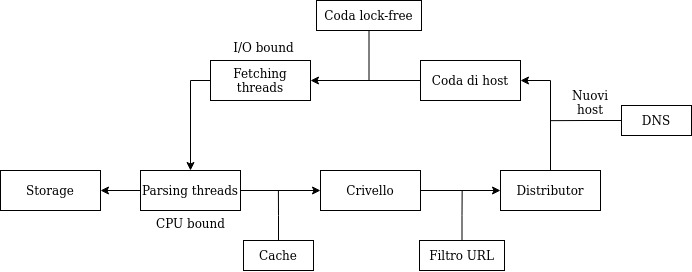
\includegraphics[width=\textwidth]{images/crawling}
    \caption{Componenti di un crawler}
\end{figure}

\subsection{Gestione parallela degli url}

\paragraph{Coordinazione agenti}
È auspicabile avere più agenti che fanno attività di crawling in parallelo, 
bisogna pensare a come distribuire il carico, un'esempio potrebbe essere quello di 
dividere per host.

Fare ciò non è molto efficiente, si può ricorrere a qualcosa di centralizzato.
Ogni agente chiede al coordinatore se tocca a lui occuparsi di un determinato host. 
Ovviamente è un single point of failure, si può pensare quindi di avere una distribuzione
del coordinatore\footnote{Un algoritmo possibile è PAXOS, una delle sue implementazioni 
è ZOOKEEPER}. Non si affronterà un algoritmo del genere, si vede ora un altro approccio.

\paragraph{Gestione statica}
Tolta la condizione di rottura degli agenti, quindi assumendo staticità, assegnare 
un url ad un agente richiede calcolare una funzione di hash modulo n, oppure 
sfruttare un approccio round robin. 

Il problema di questo approccio è che non funziona bene se gli agenti cambiano nel tempo.

\paragraph{Requisiti di gestione dinamica}

La gestione dinamica deve rispettare alcune proprietà, in particolare, si considerano
$P$ agenti, di cui $A$ agenti vivi. 

La funzione di assegnamento $\delta_A : U \rightarrow A$:
\begin{itemize}
    \item $\delta_A(u) \in A$: assegna ogni url ad un agente vivo;
    \item $\delta_A^{-1}(a) \approx \frac{|U|}{|A|}$: il carico di 
    ogni agente è circa uguale;
    \item $A \subset B \implies \delta_B^{-1}(a) \subset \delta_A^{-1}(a) \forall a \in A$: 
    aggiungendo nuovi agenti, quelli vecchi non si vedono assegnare più cose.
\end{itemize}



\paragraph{Knuth-Fisher–Yates shuffle}
Arrivato un url, creo un generatore di numeri casuali con seed pari a u. 
Permuto l'insieme $P$ di agenti e scorro finché non trovo un agente attivo $a \in A$.

Se si aggiunge un nuovo agente, gli unici url che cambiano assegnamento 
sono quelli che hanno nella lista degli agenti generata per essi, hanno un  nuovo agente che precede quello attivo selezionato precedentemente.
Quindi, gli url che cambiano posto vanno solo ad agenti nuovi.

Parto da un array lungo $n$.
Scorro l'array, all'$i$-esimo passo, seleziono una posizione $k \in [i, n-1]$ e 
scambio l'elemento $k$ e $i$.

Sono possibili $n!$ scelte, l'algoritmo genera in modo equiprobabile una permutazione possibile.

Si nota che, una volta individuato un elemento di $A$ posso fermarmi, tanto sarà
lui a gestire l'url. 
In media quindi effettuo $\frac{|A|}{|P|}$ scambi.

\paragraph{Min-hash}
Sia $u$ un url e $A$ l'insieme degli agenti, $h$ una funzione di hash. 
Un url viene assegnato all'agente $a = \argmin_{a\in A}\;h(u,a)$.

Una collisione si risolve in maniera deterministica. Questo e l'approccio
precedente sono molto simili.

\paragraph{Hashing coerente}
Un'interpretazione geometrica  è  la seguente: 
si considera una circonferenza, per ogni agente si inseriscono $C$ punti casuali 
sulla circonferenza. 
Ogni agente inizializza un seed con l'identificativo degli altri, 
generando casualmente i loro punti, quindi ogni agente ha la stessa circonferenza 
con $C$ punti per ogni $a \in A$.

Per capire dove va un url $u$, si parte dal punto definito da $h(u)$, si procede in senso orario finché non si incontra un agente.
Le repliche servono a rendere più bilanciati gli assegnamenti.

\begin{remark}
    È possibile in generale capire chi si occupava dell'url prima dell'arrivo di un 
    nuovo agente, l'approccio cambia a seconda della tecnica di hashing utilizzata, 
    nello shuffle basta procedere con l'estrazione, nel min-hashing si può mantenere 
    una finestra di k minimi. Nell'ultimo caso si può procedere nello scan della 
    circonferenza. 
\end{remark}
\newpage
